\documentclass[12pt]{article} 

%?? paths
\newcommand{\CiteMathPackage}{../../math} 
\newcommand{\CiteReference}{../reference.bib}

%?? packages 
\usepackage{setspace,geometry,fancyvrb,rotating} 
\usepackage{marginnote,datetime,enumitem} 
\usepackage{titlesec,indentfirst} 
\usepackage{amsmath,amsfonts,amssymb,amsthm,mathtools} 
\usepackage{threeparttable,booktabs,adjustbox} 
\usepackage{graphicx,epstopdf,float,soul,subfig} 
\usepackage[toc,page]{appendix} 
\usdate

%?? page setup 
\geometry{scale=0.8} 
\titleformat{\paragraph}[runin]{\itshape}{}{}{}[.] 
\titlelabel{\thetitle.\;} 
\setlength{\parindent}{10pt} 
\setlength{\parskip}{10pt} 
\usepackage{Alegreya} 
\usepackage[T1]{fontenc}
% \usepackage{fourier} % Favorite Font

%?? bibliography 
\usepackage{natbib,fancybox,url,xcolor} 
\definecolor{MyBlue}{rgb}{0,0.2,0.6} 
\definecolor{MyRed}{HTML}{D2042D}
\definecolor{MyGreen}{rgb}{0,0.4,0} 
\definecolor{MyPink}{HTML}{E50379} 
\definecolor{MyOrange}{HTML}{CC5500} 
\definecolor{MyPurple}{HTML}{BF40BF}
\newcommand{\highlightR}[1]{{\emph{\color{MyRed}{#1}}}} 
\newcommand{\highlightB}[1]{{\emph{\color{MyBlue}{#1}}}} 
\newcommand{\highlightP}[1]{{\emph{\color{MyPink}{#1}}}} 
\newcommand{\highlightO}[1]{{\emph{\color{MyOrange}{#1}}}}
\newcommand{\highlightPP}[1]{{\emph{\color{MyPurple}{#1}}}}
\usepackage[bookmarks=true,bookmarksnumbered=true,colorlinks=true,linkcolor=MyGreen,citecolor=MyGreen,filecolor=MyBlue,urlcolor=MyGreen]{hyperref} 
\bibliographystyle{econ}

%?? math and theorem environment 
\theoremstyle{definition} 
\newtheorem{assumption}{Assumption} 
\newtheorem{definition}{Definition} 
\newtheorem{theorem}{Theorem} 
\newtheorem{proposition}{Proposition} 
\newtheorem{lemma}{Lemma} 
\newtheorem{example}{Example} 
\newtheorem{corollary}[theorem]{Corollary} 
\usepackage{mathtools} 
\usepackage{\CiteMathPackage}

\begin{document} 

%??%??%??%??%??%??%??%??%??%??%??%??%??%??%??%??%??%??%??%??%??%?? 
%?? title 
%??%??%??%??%??%??%??%??%??%??%??%??%??%??%??%??%??%??%??%??%??%??

\title{\bf Secular Labor Reallocation and Business Cycles, Journal of Political Economy, 2020} 
\author{Wenzhi Wang \thanks{This note is written in my pre-doc period at the University of Chicago Booth School of Business.} } 
\date{\today} 
\maketitle 

\citet{chodorow-reichSecularLaborReallocation2020}

\section{Introduction}

Industries experience idiosyncratic shocks, genearting changes in the distribution of employment. Whether such industry labor reallocation matters quantitatively in causing, amplifying, or propagating the business cycle has important implications for our understanding of business cycles, labor markets, and the scope for policy. Yet the issue remains unsettled.

We study the consequences of \highlightB{secular labor reallocation, defined as the change in an economy's allocation of labor in response to mean-preserving, long-lasting idiosyncratic industry shocks}. We make two main contributions. First, we propose a novel method to estimate how secular labor reallocation affects local labor markets and implement it using confidential administrative employment data. Different from much of the literature exploring the ``sectoral shifts'' hypothesis, we examine whether the consequences of reallocation depend on the phase of the business cycle. We find that they do. More reallocation implies high unemployment during a recession but implies roughly neutral effects when it occurs during an expansion. Second, we show that a multiarea, multisector search-and-matching model featuring realistic frictions to sectoral mobility and downward wage rigidity can rationalize this result. 

Our analysis starts in Section 2 with a description of our empirical identification strategy. A number of challenges arise. First, the small number of national business cycles in periods with high-frequency, high-quality industry-level data limit inference based only on national variation. Second, realized reallocation within a business cycle may reflect cyclical sensitivities that vary across industries \citep{abrahamCyclicalUnemploymentSectoral1986}, and business cycles can cause permanent reallocation of inputs. Third, we generally do not observe pure cross-industry dispersion shocks that do not also affect the mean of variables such as productivity. To circumvent the small number of national business cycles, we use variation in reallocation and business cycle outcomes across broadly defined local labor markets in the United States. To isolate long-lasting shocks, our metric of reallocation sums the absolute value of industry employment share changes between the start and the end of a recession-to-recovery or expansion cycle, thereby filtering out cyclical changes that occur during a recession but reverse during a recovery. We address the endogeneity of reallocation to local conditions by developing a Bartik-style measure of predicted reallocation on the basis of a local area's initial industry composition and industyr employment changes in the rest of the country and use this measure as an instrument for actual reallocation. Finally, we account for non-mean-preserving industry shifts by directly controlling for the Bartik predicted employment growth rate given an area's industry composition. Thus, our empirical specification regresses local area unemployment on local area reallocation, controlling for predicted growth and with reallocation instrumented using predicted reallocation. Intuitively, the research design compares ourcomes in areas with the same predicted employment growth but different predicted reallocation.

We implement our exercise using confidential employment data by local area and industry from the BLS Longitudinal Database (LDB) merged with the public-use counterpart of these data, the Quarterly Census of Employment and Wages (QCEW). We use the public-use version to extend the analysis back to 1979. The resulting data set tracks industry reallocation in more than 200 urban local labor markets.

Section 4 contains our empirical analysis. Predicted reallocation is a strong instrument for actual reallocation except around the 199 recession because of a change in the data collection procedure at that time. We therefore introduce a two-sample two-stage least squares (TS2SLS) design where we estimate the first stage excluding the 1990 episode but include it in the second stage and derive the standard error formula appropriate to this setting. Our formula should prove useful in other settings where researchers encounter missing data. 

We obtain two main empirical results. First, high reallocation causes higher unemployment. Second, this average response masks a crucial asymmetry. During a recession-to-recovery cycle, a 1 standard deviation increase in predicted reallocation raises unemployment by roughly $0.5$ percentage points at the national recession trough, with the effect then dissipating over the subsequent recovery. In contrast, reallocation does not affect unemployment during an expansion. These results are statistically strong, are not driven by particular sectors or areas, and are robust to inclusion of local area time-varying control variables or local area fixed effects.

Section 5 introduces a multiarea, multisector model of reallocation and unemployment to provide a structural interpretation of our results. Each area in the model contains a number of industries consisting of firms and workers who interact according to a search-and-matching framework subject to a downward nominal wage constraint. The shares of workers and firms in each industry depend on industry-specific productivity and consumer preferences. In line with the data, the model features two-wage gross flows of workers across industries in each period. We shock the model with an increase in the cross-sectional variance of industry-level productivities and estimate the same regression in the model as in the data. Specifically, we estimate the marginal effect of reallocation on unemployment during an expansion -- in which the increase in the cross-sectional variance of industry productivity consistitutes the only set of shocks -- and a recession -- in which borrowers simultaneously face an increase in the interest rate. 

Without any labor market or wage-setting frictions, reallocation across industries would occur instantaneously and without generating any unemployment. Allowing for only within-industry search-and-matching frictions, the mean preserving spread in industry productivities generates a small increase in unemployment regardless of whether it occurs coincident with a demand-induced recession. Incorporation of frictions to moving across industries and empirically plausible downward wage rigidity breaks this symmetry. \highlightP{Intuitively, during expansions higher wages draw job seekers into the expanding sectors, while wage compression during recessions pushes the adjustment into a greater difference in job-finding rates.} We construct impulse response functions of the cross-area marginal effect of reallocation on unemployment in model-simulated data and find that they accord well with their empirical results. 

\section{Measurement and Empirical Strategy}

We define a measure of reallocation across industries and then discuss our empirical strategy.

\subsection{Measure of Reallocation}

We define an index of reallocation based on the dispersion in industry employment growth rates as in \citet{lilienSectoralShiftsCyclical1982}. The economy consists of $A$ areas, each with $I$ industries. Let $e_{a, i, t}$ denote employment in area $a$ and industry $i$ at time $t$, $e_{a,t} = \sum_{i=1}^{I} e_{a, i, t}$ total employment in the area, $s_{a,i,t} = e_{a,i,t} / e_{a,t}$ industry $i$'s employment share, $g_{a, i, t, t+j} = e_{a, i, t+j} / e_{a, i, t} - 1$ the area-industry employment growth rate, and $g_{a, t, t+j} = e_{a, t+j} / e_{a, t} - 1$ total local area employment growth. Reallocation in area $a$ between months $t$ and $t+j$ is 
\begin{equation}
    \label{chodorow-reichSecularLaborReallocation2020_eq1}
    R_{a, t, t+j} = \frac{12}{j} \frac{1}{2} \sum_{i}^{I} s_{a, i, t} \abs{\frac{1 + g_{a, i, t, t+j}}{1 + g_{a, t, t+j}} - 1}.
\end{equation} 

The measure $R_{a, t, t+j}$ is easily interpreted. The term $1/2 \sum_{i=1}^{I} \abs{\bp{1 + g_{a, i, t, t+j}} / \bp{1 + g_{a, t, t+j}} - 1}$ equals zero if employment grows at an identical rate in every industry between $t$ and $t+j$ and one if all industries with positive employment in $t$ disappear by $t+j$. In general, this term is between zero and one, with higher realizations indicating more reallocation. The ratio $12/j$ translates the reallocation between $t$ and $t+j$ into an annualized monthly flow, such that $R_{a, t, t+j} \subset \bs{0, 12/j}$.

\subsection{Econometric Approach}

We assume that unemployment and reallocation in local area $a$ evolve according to 
\begin{equation}
    \label{chodorow-reichSecularLaborReallocation2020_eq2}
    \D u_{a, t, t+j} = \b_j R_{a, t, t+k} + \Gc\of{\bc{s_{a, i, t}}; \bc{\eta_{i, t, t+j}}} + \G^{u^{\prime}} X_{a, t} + \ve_{a, t, t+j},
\end{equation}
\begin{equation}
    \label{chodorow-reichSecularLaborReallocation2020_eq3}
    R_{a, t, t+k} = \Cc\of{u_{a,t}, u_{a, t+1}, \ldots, u_{a, t+k}} + \Rc\of{\bc{s_{a, i, t}}; \bc{\eta_{i, t, t+k}}} + \G^{R^{\prime}} X_{a, t} + \nu_{a, t, t+k},
\end{equation}
where $\D u_{a, t, t+j} = u_{a, t+j} - u_{a, t}$, $\Gc\of{\bc{s_{a, i, t}}; \bc{\eta_{i, t, t+j}}}$, and $\Rc\of{\bc{s_{a, i, t}}; \bc{\eta_{i, t, t+k}}}$ are functions that relate cumulative idiosyncratic industry-level shocks $\bc{\eta_{i, t, t+k}}$ and local area employment shares to local area unemployment and reallocation; $X_{a,t}$ contains time $t$ measurable observed variables that affect unemployment or reallocation; and $\ve_{a, t, t+j}$ and $\nu_{a, t, t+k}$ are unobserved area-specific determinants. We write $\eta_{i, t, t+k}$ without $a$ subscript to emphasize that these shocks occur at the national level; shocks to an industry specific to a particular area are subsumed in $\nu_{a, t, t+k}$. While we do not need to specify the functions forms of $\Gc$ and $\Rc$, it is natural and convenient to think of $\Gc$ as a function solely of the weighted mean shock in an area $\sum_{i} s_{a, i, t} \eta_{i, t, t+j}$ and $\Rc$ as a function of the weighted dispersion in $\bc{\eta_{i, t, t+k}}$.

Our object of interest is $\b_j$, the effect of reallocation on unemployment. Previous literature has emphasized two sources of causality running instead from unemployment to reallocation, captured by $\Cc\of{\cdot}$ function in equation (\ref{chodorow-reichSecularLaborReallocation2020_eq3}). First, a low opportunity cost of restructuring during periods of high unemployment and weak demand may lead to higher reallocation. Second, a demand-induced recession can cause cyclical reallocation across industries if industries differ in their cyclical sensitivities \citep{abrahamCyclicalUnemploymentSectoral1986}. More generally, both unemployment and reallocation may depend on common determinants, as captured by the common arguments in the $\Gc$ and $\Rc$ functions. For example, an area with a large manufacturing base in 1980 may have had high unemployment directly as a result of concentrating in industries that had negative labor demand shocks while also experiencing substantial reallocation over the past few decades.

\paragraph{Double Bartik} We introduce a ``double Bartik'' strategy to overcome these difficulties. We define Bartic predicted employment growth as the employment growth in local area $a$ if employment in each local industry grew at exactly the same rate as employment in that industry in the rest of the country.
\begin{equation}
    \label{chodorow-reichSecularLaborReallocation2020_eq4}
    g_{a, t, t+j}^{b} = \frac{12}{j} \sum_{i=1}^{I} s_{a, i, t} g_{-a, i, t, t+j},
\end{equation}
where $e_{-a, i, t}$ denotes employment in industry $i$ at time $t$ summing over all areas other than area $a$ and $g_{-a, i, t, t+j} \coloneqq e_{-a, i, t+j} / e_{-a, i, t} - 1$ is the leave-one-out employment growth rate for industry $i$. Substituting $g_{-a, i, t, t+j}$ and $g_{a, t, t+j}^{b}$ into equation (\ref{chodorow-reichSecularLaborReallocation2020_eq1}), we analogously define Bartik predicted reallocation as the reallocation that would be obtained in area $a$ if employment in each local industry grew at exactly the same rate as employment in that industry in the rest of the country, 
\begin{equation}
    \label{chodorow-reichSecularLaborReallocation2020_eq5}
    R_{a, t, t+k}^{b} = \frac{12}{k} \bp{\sum_{i=1}^{I} s_{a,i,t} \abs{\frac{1 + g_{-a, i, t, t+k}}{1 + g_{a, t, t+k}^{b}} - 1}}.
\end{equation} 
We believe this second Bartik measure is original.

\highlightPP{We use Bartik predicted reallocation $R_{a, t, t+k}^b$ as an excluded instrument for $R_{a, t, t+k}$ and Bartik predicted employment growth as a control (i.e., included instrument) in a specification including period fixed effects.} To understand this specification, suppose that we knew the functions $\Gc$ and $\Rc$ and observed $\bc{\eta_{i, t, t+k}}$. Then, so long as $\Gc$ and $\Rc$ were not collinear, estimating equations (\ref{chodorow-reichSecularLaborReallocation2020_eq2}) and (\ref{chodorow-reichSecularLaborReallocation2020_eq3}) with $\Rc$ as an excluded instrument and $\Gc$ as an included instrument would identify $\b_j$ from the part of local reallocation due to $\Rc$ and after controlling for the direct effect of industry shocks on local are unemployment that occur through the function $\Gc$. Since we do not actually observe these shocks or know these functions, we assume instead that Bartik growth and reallocation, measured over appropriate time spans, can proxy for the functions $\Gc$ and $\Rc$. 

Indeed, Bartik reallocation being a good proxy for $\Rc$ implies the relevance condition $$\cov\of{R_{a, t, t+k}, R_{a, t, t+k}^b \mid g_{a, t, t+k}^b, X_{a, t}, \a_{t}} > 0.$$ The exclusion restriction $$\cov\of{\ve_{a, t, t+j}, R_{a, t, t+k}^b \mid g_{a, t, t+k}^b, X_{a, t}, \a_{t}} = 0$$ requires that Bartik growth absorb all direct effects of industry shocks on unemployment that occur through $\Gc$. Furthermore, specifying predicted reallocation as an excluded instrument solves the problem of feedback from local unemployment to reallocation because (with time fixed effects) predicted reallocation does not depend on local outcomes after time $t$, while including $g_{a, t, t+k}^{b}$ controls for both the area's industrial cyclical sensitivity and the possibility that predicted real-location concentrates in areas also undergoing secular decline or expansion. \highlightP{Intuitively, the research design compares areas with the same predicted growth but different predicted allocation. }

\paragraph{Reallocation timing} 

If labor market frictions impede reallocation, then the pattern of national industry employment growth could lag shifts in $\bc{\eta_{i, t, t+k}}$ and make Bartik growth and reallocation, which depend on realized national industry employment growth rates, poor proxies for the functions of the underlying shocks. To address this potentiality, we measure both actual and predicted reallocation over two separate, multi-period windows. The first window begins at a national employment peak and lasts through the course of a national recession and subsequent labor market recovery. The second window begins when the labor market has fully recovered and ends at the start of the next recession. Therefore, we assume that actual national employment reallocation between the start and the end of a recession-to-recovery cycle and over an expansion fully reflects the reallocation that would eventually occur as a result of the idiosyncratic industry shocks, so that the Bartik reallocation instrument embodies the reallocation in an area implied by the national industry shocks. This timing also filters out temporary reallocation induced by differing cyclical sensitivities.

\highlightPP{We define a national labor market recession as the period between a private sector employment peak and the employment trough, a recovery as the period from the trough until the economy regains its previous peak level, and an expansion as the period between the end of a recovery and the start of the next recession.} Thus, we measure reallocation over the 2005-8 expansion using the growth rates of industry employment between June 2005 and the private sector employment peak in January 2008 and reallocation during the 2008-14 recession-to-recovery cycle using the growth rates of industry employment between January 2008 and March 2014 when employment first regains its January 2008 level. Figure \ref{chodorow-reichSecularLaborReallocation2020_fig1} illustrates the labor market recessions, recoveries, and expansions in our sample. (We treat the 1980-82 period as a single long recession.) The view of cyclical tightness as the same at the start and the end of each recession-to-recovery and expansion cycle echoes the ``gaps'' view of business cycles advocated by DeLong and Summers (1988). Our main results are not sensitive to this particular partitioning. We apply the same national timing to all local areas to compute predicted and realized reallocation, allowing for the interpretation of our regressions as pooled cross sections.

\begin{figure}[H]
    \noindent\caption{National business cycle partition}
    \begin{center}
        \resizebox{1\textwidth}{!}{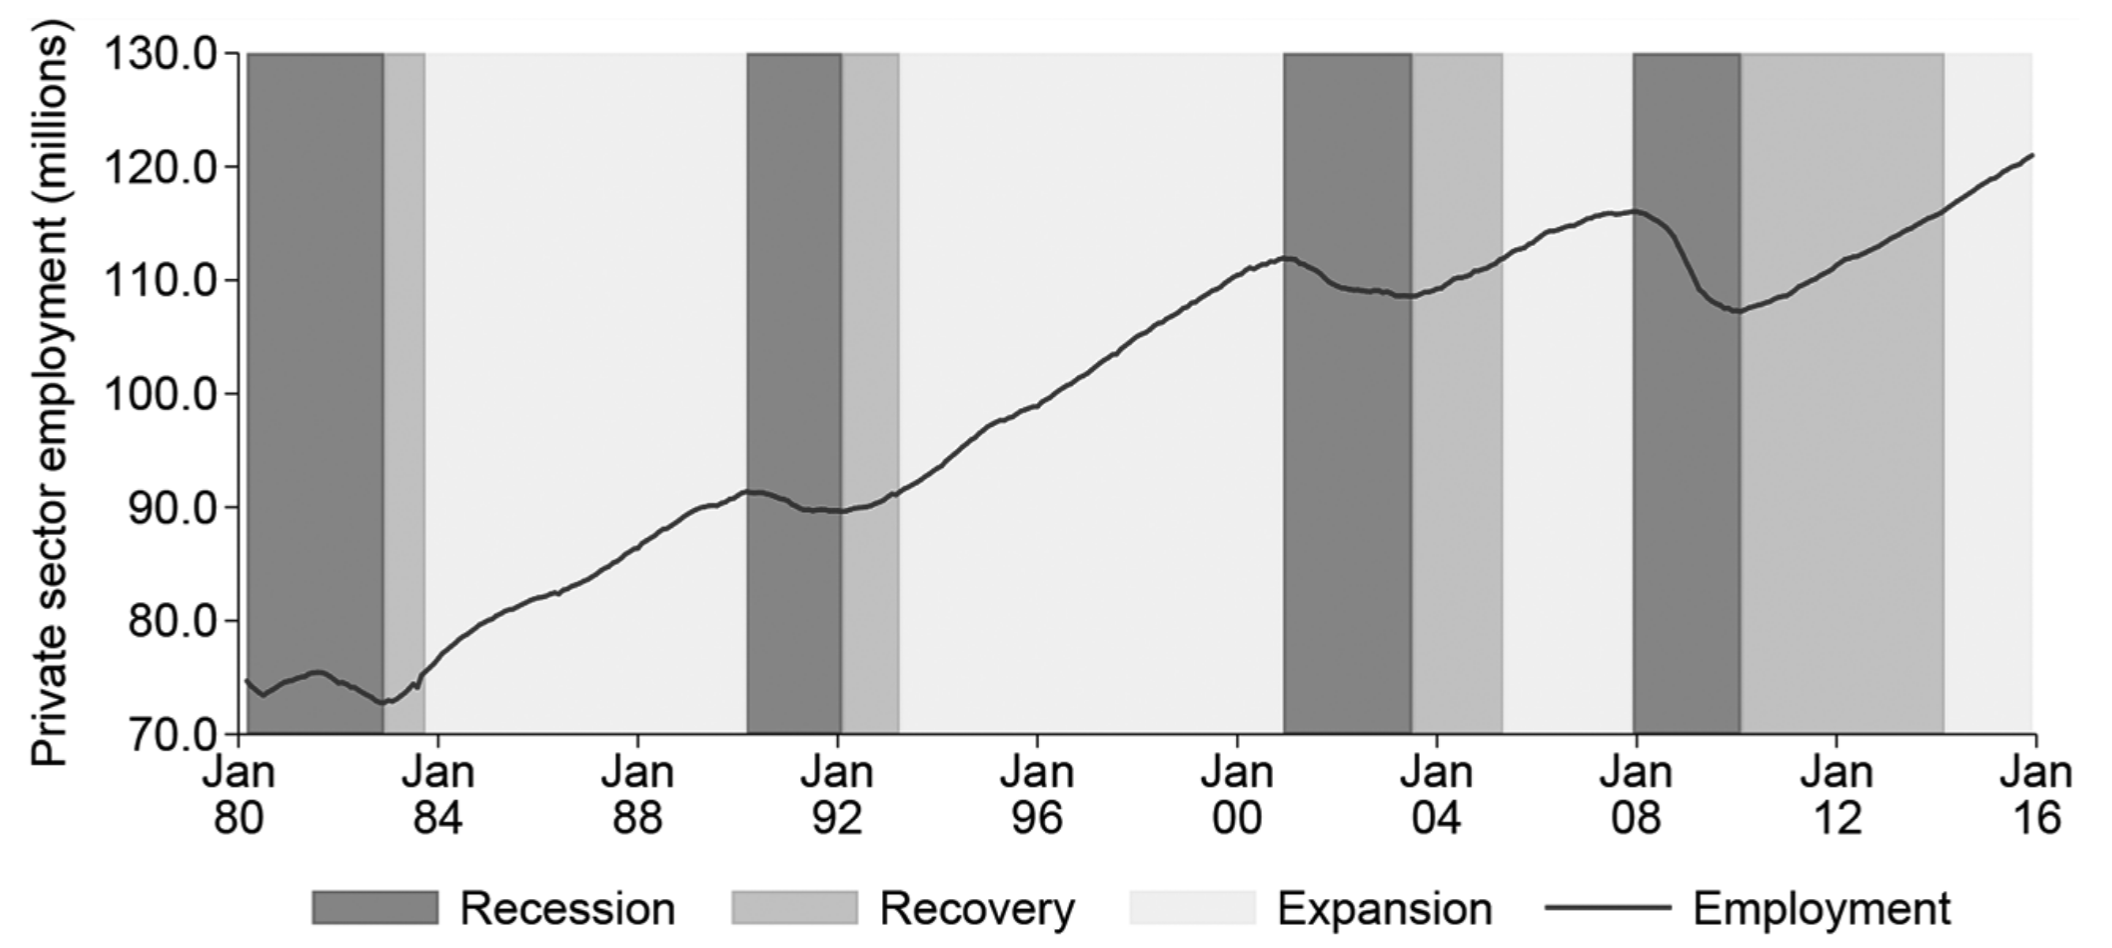
\includegraphics{chodorow-reichSecularLaborReallocation2020_fig1.png}}
        \label{chodorow-reichSecularLaborReallocation2020_fig1}
    \end{center}
\end{figure}

By construction, national reallocation during a recession-to-recovery cycle is mean preserving in overall employment. Measuring reallocation between two periods when total employment remains unchanged facilitates a natural economic interpretation, since 
\begin{equation}
    \label{chodorow-reichSecularLaborReallocation2020_eq6}
    R_{a, t, t+T} \mid_{e_{a,t} = e_{a, t+T}} = \frac{12}{T} \frac{1}{2} \sum_{i=1}^{I} \abs{\frac{e_{a, i, t+T} - e_{a, i, t}}{e_{a, t}}}.
\end{equation}
Equation (\ref{chodorow-reichSecularLaborReallocation2020_eq6}) rewrites $R_{a, t, t+T}$ as the minimum fraction of total period $t$ employment that changes industries between $t$ and $t+T$, expressed as a monthly flow at an annual rate. When ${e_{-a,t} = e_{-a, t+T}}$, a derivation similar to equation (\ref{chodorow-reichSecularLaborReallocation2020_eq6}) shows that predicted reallocation $R^b_{a, t, t+T}$ has the interpretation of the predicted net quantity of industry employment reshuffling between $t$ and $t+T$ as a share of total employment at $t$, expressed at an annual rate. 


\paragraph{Other specification details} An important element of our analysis will be to allow the effect of reallocation on unemployment to vary by the phase of the business cycle. We argue in section 5 that the differences in $\b$ across business cycle phases are informative about the underlying economic mechanisms.

Finally, varying the horizon of the unemployment response and holding fixed the horizon over which the reallocation occurs traces out an impulse response function. That is, for months $t$ that mark the start of a recession or an expansion and letting $T$ dentoe the length of the recession-to-recovery cycle or the expansion, we estimate for $c \in \bc{\text{Recession-to-recovery}, \text{Expansion}}$,
\begin{equation}
    \label{chodorow-reichSecularLaborReallocation2020_eq7}
    \D u_{a, t, t+j} = \b_{j, c} R_{a, t, t+T} + g_{a, t, t+T}^b + \G_{j, c}^{u^{\prime}} X_{a, t} + \ve_{a, t, t+j}.
\end{equation}

\subsection{Discussion}

The Bartik research design has the advantage of not requiring the researcher to take a stand on the deep industry-level determinants of reallocation in any given period (the $\eta_i$ in our notation), such as changes in technology, consumer tastes, exchange rates, or trade policy. Rather, the evolution of employment nationally summarizes the consequences of the combination of these deep determinants for reallocation. \highlightP{The Bartik approach simply requires that the deep determinants produce a common component of industry employment growth across areas and that, after residualizing with respect to predicted area growth, these determinants affect local areas only through their effect on reallocation.} Not needing to link reallocation to a primitive shock makes this approach well suited to the study of business cycle frequency outcomes that span multiple cycles, each with its own unique deep determinants of reallocation.

This aspect of the research design also introduces two important limitations. First, we study the consequences of reallocation but do not attempt to identify its primitive causes and therefore cannot answer how a policy maker might manipulate reallocation if desired. Related, the representation (\ref{chodorow-reichSecularLaborReallocation2020_eq2}) and (\ref{chodorow-reichSecularLaborReallocation2020_eq3}) may not uniquely characterize the system, as unemployment ultimately depends on the underlying shocks. Nonetheless, our results shed light on a long-running debate about whether the frictional reallocation of labor exerts an independent impact on unemployment and the frictions that give rise to such effects. Second, despite the common usage of the phrase ``Bartik shock'' (which we have purposefully avoided), neither Bartik predicted employment growth nor predicted reallocation necessarily constitutes a shock in the standard meaning of being unanticipated and orthogonal to previous outcomes. In our setting, anticipation effects -- knowledge of the industry shocks $\bc{\eta_{i, t, t+k}}$ before time $t$ -- would complicate the interpretation of $\b$ if unemployment begins to rise before the reallocation occurs. In our empirical work, we test for differential pretrends to diagnose such anticipation effects and find little evidence for them. The model in section 5 expands on both of these issues by providing a concrete example of a set of primitive shocks $\bc{\eta_{i, t, t+k}}$ that give rise to our measure of reallocation. 


\section{Data and Summary Statistics}

\subsection{Data}

Data on employment by county and industry come from the BLS LDB and the QCEW. The LDB reports employment by establishment and month starting in 1990. The source data come from quarterly reports that employers file with state employment security agencies as part of the unemployment insurance system; as a result, the LDB contains essentially universal coverage of private-sector employment. Each establishment in the LDB has a six-digit North American Industry Classification System (NAICS) code associated with its primary activity. Our LDB sample contains 42 states that allow access to their data through the BLS visiting researcher confidential data access program. These data are uniquely suited to measuring reallocation because they do not contain sampling error, which would artificially increase reallocation rates.

The QCEW is the public-use version of the LDB. It reports monthly employment at the industry-county level for all 50 states starting in 1975, subject to disclosure limitations to prevent the release of identifying information regarding single establishments. We use the QCEW to extend the sample back to 1979 and to fill in states not in our LDB sample.

Two details of the data collection procedure merit mention as they affect our analysis. First, the Federal Unemployment Compensation Amendments of 1976 expanded the number of industries and establishments covered by unemployment insurance laws, with the result that the QCEW expanded its coverage of employment between 1976 and 1980. We exclude data before 1978 because the staggered implementation of the coverage expansion across states produces substantial measurement difficulties during that period. In effect, we exclude the 1976-80 expansion from the analysis. Second, in 1990 and 1991 the BLS lowered the threshold requirements for multiestablishment employers to report employment by single establishment. As a result, an unusually high number of establishments changed industry code during those years. While predicted reallocation during the 1990-93 recession-to-recovery cycle should remain mostly unaffected by the reclassifications as long as the changes roughly net out at the national level, actual reallocation at the local level has sufficient measurement error to render it unusable. We instead develop a TS2SLS estimator, where we estimate the first stage excluding the 1990-93 period as described further below.

We combine the LDB data with NAICS three-digit employment from the QCEW for counties in states that are not in the LDB and with two-digit Standard Industrial Classification (SIC) data for 1975-2000. \highlightPP{We seasonally adjust all series at the industry-county level using the multistep moving average approach contained in the Census Bureau's X-11 algorithm.} Relative to other data sets with employment by geography and industry, such as the Census Bureau's County Business Patterns or Longitudinal Business Database (LBD), the BLS data have the important advantage for business cycle analysis of providing monthly rather than annual frequency. We choose SIC 2/NAICS 3 as our level of industry detail because our measure of reallocation does not distinguish between movement across similar or dissimilar industries. The SIC 2/NAICS 3 level allows for enough industry detail (roughly 80 industries) to generate variation in reallocation across areas while ensuring that all such reallocation occurs across broadly defined industries. A finer level of detail would also diminish our ability to make any use of the public data.

We aggregate county-level data into core-based statistical areas (CBSAs) using the 2013 Office of Management and Budget (OMB) county classifications. The OMB defines CBSAs as areas ``containing a large population nucleus and adjacent communities that have a high degree of integration with that nucleus'' and distinguishes between metropolitan (MSA) and micropolitan (MiSA) areas depending on whether the urban core contains at least 50,000 inhabitants. We further aggregate CBSAs into combined statistical areas (CSAs). CSAs consist of adjacent CBSAs that have ``substantial employment interchange'' and thus better capture the local labor market. Not all CBSAs belong to a CSA. For example, the San Diego MSA is not part of a CSA, but the Boston-Cambridge-Newton MSA is one of five MSAs in the Boston-Worcester-Providence CSA.


Our main outcome variable is the local unemployment rate and comes from the BLS Local Area Unemployment Statistics (LAUS) program. We combine published data starting in 1990 with unpublished data available from the LAUS office for 1976-89. For 1990-present, the LAUS office provides seasonally adjusted data for MSAs; we augment these data by seasonally adjusting the county data using the same procedure described above for the 1976-89 period and for counties not in an MSA and aggregate up to the MSA or CSA level. While the construction of county and MSA unemployment rates involves imputation, any noise is likely to be classical left-hand-side error, and the unemployment rate offers conceptual advantages by reducing the effect of migration on the analysis.

Our final sample includes all MSAs and CSAs containing at least one MSA, with employment of at least 50,000 in 1 month, an agricultural share of employment of less than 20\%, and where we observe at least 95\% of private-sector employment at the industry level. The final sample contains $1,314$ of the $3,144$ counties in the United States and covers $86\%$ of 2013 employment.

\subsection{Trends in National Reallocation}

An overview of reallocation at the national level provides useful context for what follows. Table 1 reports national reallocation, $R_{US, t, t+j}$, for each recession-to-recovery cycle and expansion and at various levels of industry aggregation. The rows with all data in boldface indicate the recession-to-recovery episodes. We measure reallocation using SIC definitions for the episodes between 1975 and 2000 and using NAICS definitions for the episodes beginning after 1990.

A number of interesting patterns emerge. First, cross-industry reallocation occurs all the time. Since \citet{lilienSectoralShiftsCyclical1982}, a debate has continued about whether sectoral employment shifts concentrate enough during periods of low economic activity to explain fluctuations in the business cycle. The problem identified by \cite{abrahamCyclicalUnemploymentSectoral1986} of how to account for different industry cyclical sensitivities during recessions makes answering this question difficult. By filtering out cyclical reallocation that occurs during a recession but reverts during a recovery, our timing approach provides one way around the \citet{abrahamCyclicalUnemploymentSectoral1986} critique. Using our approach, more secular reallocation does occur during episodes containing recessions, qualitatively consistent with the \citeauthor{lilienSectoralShiftsCyclical1982} conjecture.

Second, consistent with a downward trend in a number of measures of labor market flows, the rate of reallocation has trended down. For example, $4.6\%$ ($1.29 \times 43/12$) of employment changed SIC two-digit industry between March 1980 and October 1983. The same fraction changed NAICS threedigit industry between January 2008 and February 2014, despite the latter recession-to-recovery episode lasting $30$ months longer. As a result, monthly reallocation fell from $1.29\%$ (at an annual rate) during the 1980-83 episode to $0.74\%$ during the 2008-14 episode. The decline in between is monotonic for recession-to-recovery cycles. Despite the widespread attention to industry reallocation during the 2008-14 episode, our measure of secular reallocation suggests a decline in reallocation intensity during the Great Recession period.

Third, a large amount of reallocation occurs across broadly defined industries. For example, of the $6.5\%$ ($1.06\%$ per year multiplied by $6.08$ years) of employment changing six-digit NAICS industry between January 2008 and March 2014, $4.1$ percentage points constituted movement across twodigit industries.

Fourth, while individual industries exhibit persistence in their contribution to national reallocation, the explanatory power of this relationship lies well below one. We establish this fact by reporting in the penultimate line of the table the $R^2$ values from the regression $j^{-1} \abs{\D s_{i, t, t+j}} = \a_i + \ve_{i, t}$. For example, at the NAICS 3 level, the $R^2$ value of this regression is $0.59$. Thus, individual industry trends leave unexplained $40\%$ of the variation in the contribution of industries to national reallocation. This time variation in industry employment trends will in turn contribute to substantial variation over time in the predicted reallocation in individual areas.

\renewcommand{\thefigure}{Table \arabic{figure}}
\setcounter{figure}{0}   
\begin{figure}[H]
    \noindent\caption{Reallocation by episode and industry detail}
    \begin{center}
        \resizebox{1\textwidth}{!}{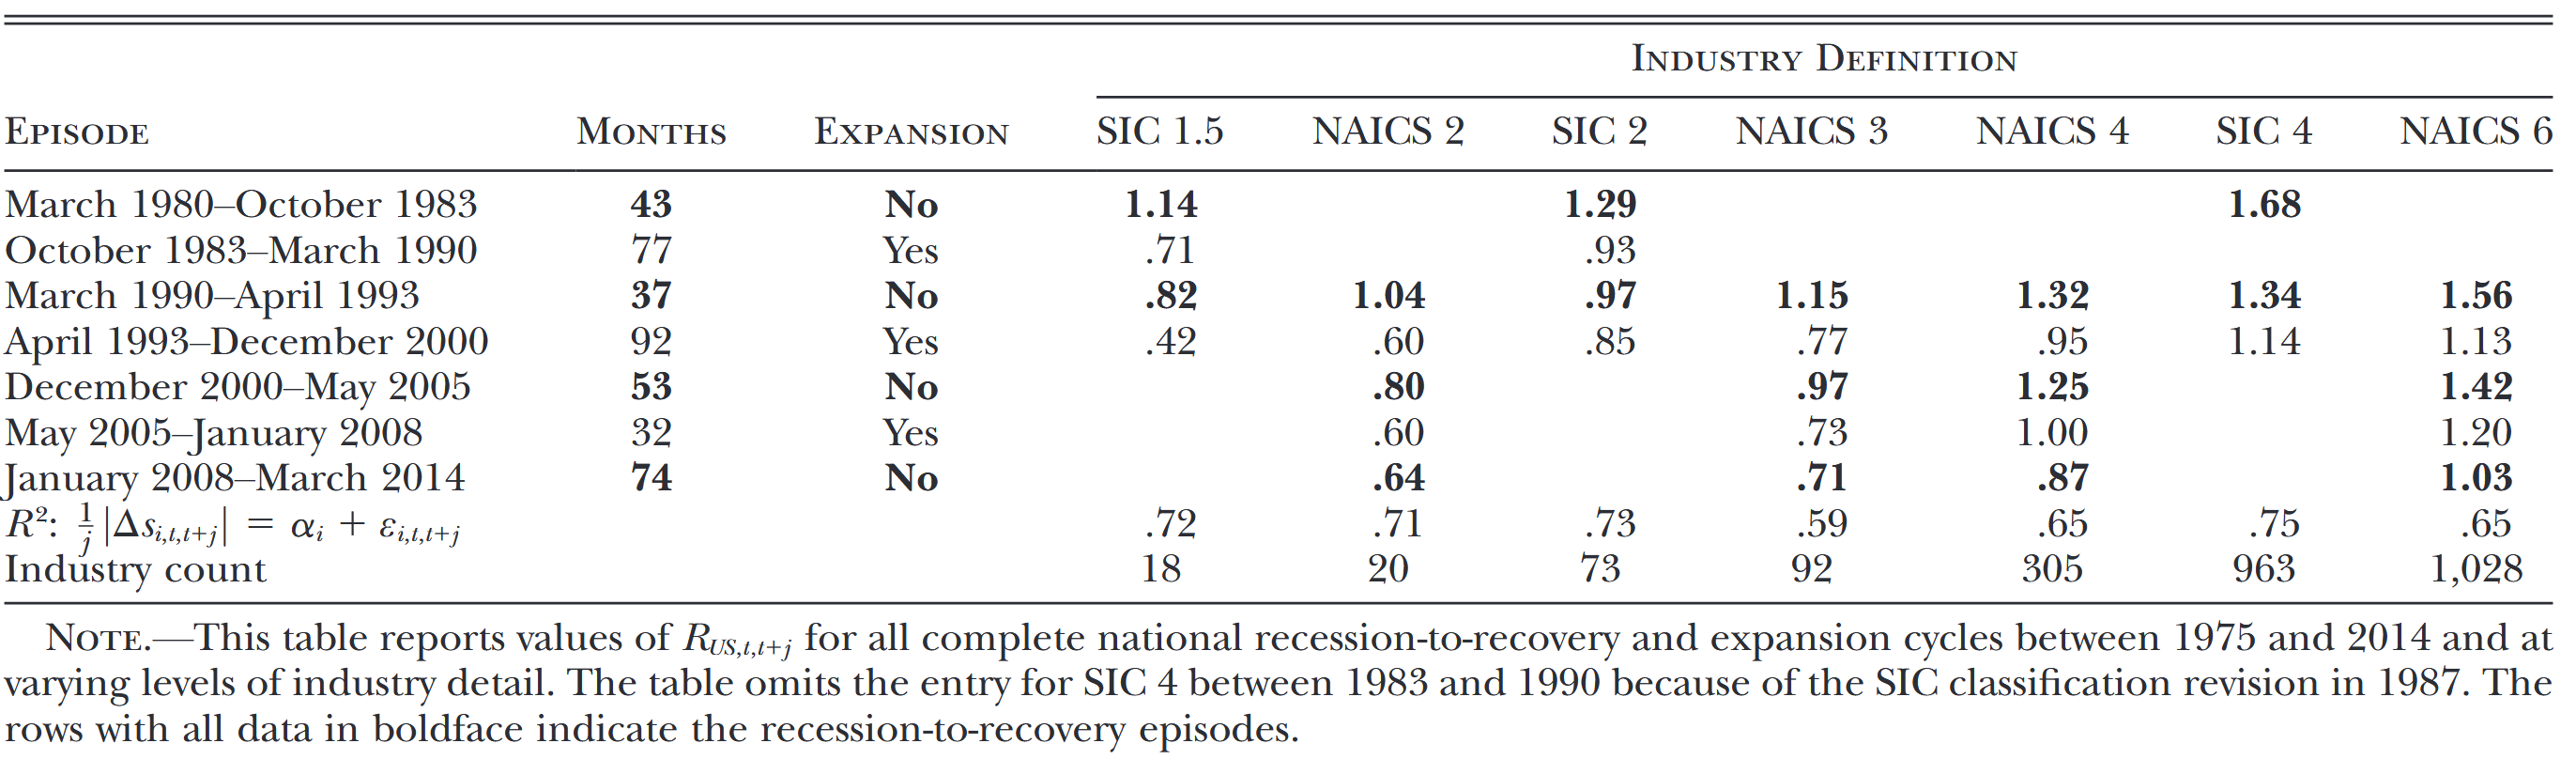
\includegraphics{chodorow-reichSecularLaborReallocation2020_tab1.png}}
        \label{chodorow-reichSecularLaborReallocation2020_tab1}
    \end{center}
\end{figure}

\subsection{Local Reallocation}

Figure \ref{chodorow-reichSecularLaborReallocation2020_fig2} shows a map of the variation in predicted reallocation during the 2008-14 recession-to-recovery cycle. We split the MSA/CSA observations into quintiles based on their Bartik reallocation and mark higher reallocation levels with darker shading. The map shows that predicted reallocation is not easily explained by geographic factors.

\renewcommand{\thefigure}{\arabic{figure}}
\setcounter{figure}{1}   
\begin{figure}[H]
    \noindent\caption{Map of predicted reallocation per year, 2008-14 cycle}
    \begin{center}
        \resizebox{1\textwidth}{!}{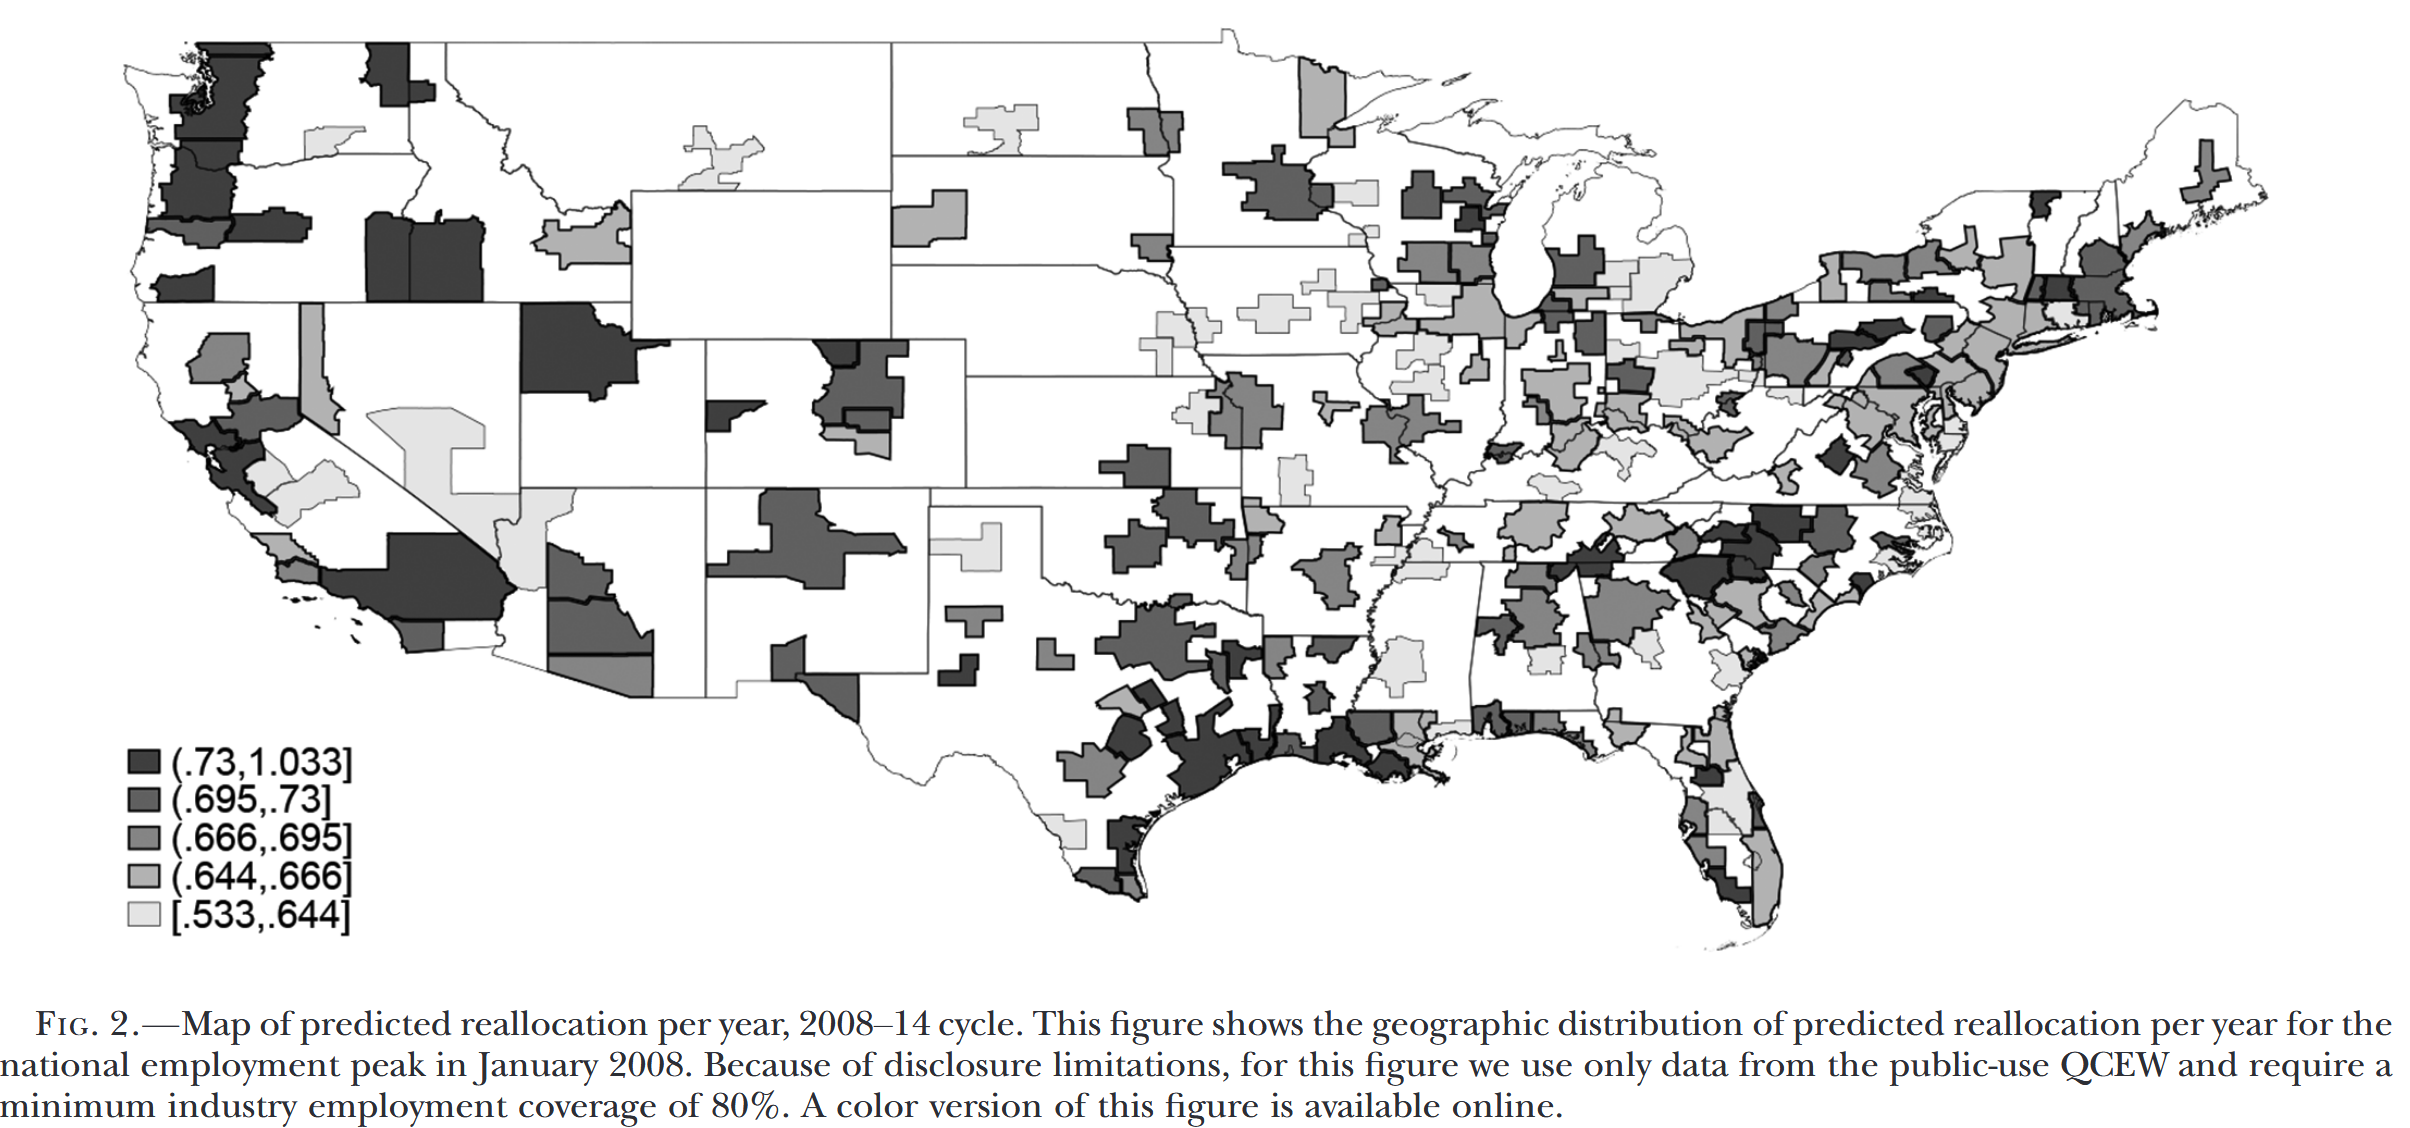
\includegraphics{chodorow-reichSecularLaborReallocation2020_fig2.png}}
        \label{chodorow-reichSecularLaborReallocation2020_fig2}
    \end{center}
\end{figure}

\renewcommand{\thefigure}{Table \arabic{figure}}
\setcounter{figure}{1}   
\begin{figure}[H]
    \noindent\caption{Correlation of predicted reallocation across episodes}
    \begin{center}
        \resizebox{1\textwidth}{!}{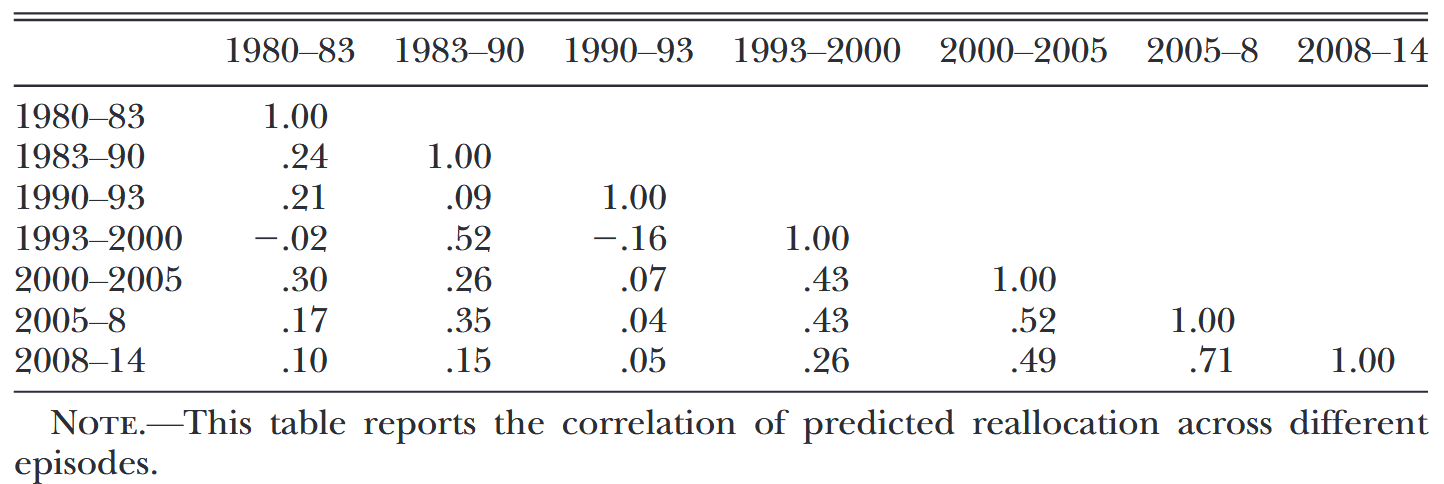
\includegraphics{chodorow-reichSecularLaborReallocation2020_tab2.png}}
        \label{chodorow-reichSecularLaborReallocation2020_tab2}
    \end{center}
\end{figure}

\ref{chodorow-reichSecularLaborReallocation2020_tab2} reports the pairwise correlations in predicted local reallocation across each national recession-to-recovery and expansion cycle. Predicted reallocation has a modest correlation across most episodes. These patterns inform our analysis in three ways. First, in some specifications we will exploit the absence of perfect serial correlation by including area fixed effects. Second, we will always cluster all standard errors by CSA/MSA to account for arbitrary correlation within an area over time. Third, in interpreting our findings and in the model in section 5, we will not assume that reallocation at the start of a cycle is unanticipated.

\section{Empirical Results}

\subsection{First-Stage and Two-Sample 2SLS}

\subsection{Effects of Reallocation}

\subsection{Robustness}

\section{Quantitative Model}

The previous section demonstrated that reallocation causes an increase in unemployment if it occurs during a national recession-to-recovery cycle but not if it occurs during an expansion. The rise in the unemployment rate concentrates during the recession part of the cycle, with maximum impact around the national employment trough. We now study a model economy to better understand these patterns. The model illustrates what types of primitive shocks could give rise to our empirical setup and how frictions to labor mobility and downward wage rigidity allow the model to match the empirical patterns in the data.

\subsection{Setup}

Time is discrete. The economy consists of $\Ac$ islands, each of which has $\Ic$ industries. We assume no aggregate uncertainty and perfect consumption insurance within (but not across) islands, which implies an island-specific discount factor $m_{a, t, t+1}$.

\subsubsection{Labor Market}

The labor market in each area-industry operates according to search-and-matching principles. At the beginning of period $t$, industry $i$ in area $a$ contains $\bp{1-\d_{t-1}} e_{a, i, t-1}$ workers employed in the previous period and still attached to their firm, $x_{a, i, t}$ workers searching for a job, and $v_{a, i, t}$ job vacancies. Hiring occurs at the beginning of the period, with $n_{a, i, t}$ new matches formed. The $e_{a, i, t} = \bp{1 - \d_{t-1}} e_{a, i, t} + n_{a, i, t}$ workers employed in $t$ engage in production. At the end of the period, $\d_t e_{a, i, t}$ of the employed workers exogenously separate from their employer. We le $u_{a, i, t} = x_{a, i, t} - n_{a, i, t}$ denote the number of unemployed workers in period $t$ after the matching process has taken place. This concept of unemployment allows for job-to-job transitions by workers who separate at the end of $t-1$ but get newly hired at the beginning of $t$. We let $l_{a,i,t} = e_{a,i,t} + u_{a, i, t} = \bp{1 - \d_{t-1}} e_{a, i, t-1} + x_{a, i, t}$ denote the total labor force in industry $i$ in area $a$ at time $t$. We fix the economy-wide labor force at $\sum_{a \in \Ac} \sum_{i \in \Ic} l_{a, i, t} = 1$.

The firm vacancy-posting condition and matching process are standard. Firms post $v_{a,i,t}$ vacancies in industry $i$ at cost $\kappa$ per vacancy. A freeentry condition drives the expected value of a vacancy to zero. The matching function takes the Cobb-Douglas form $n_{a, i, t} = M v_{a, i, t}^{1-\a} x_{a,i,t}^{\a}$. Letting $\t_{a,i,t} = v_{a,i,t} / x_{a,i,t}$ denote the vacancy-searcher ratio, or industry market tightness, searching workers find jobs at rate $f_{a,i,t} = M \t_{a,i,t}^{1-\a}$, and firms fill vacancies at rate $q_{a,i,t} = M \t_{a,i,t}^{-\a}$. Thus, the value of a filled job to the firm, $J_{a,i,t}$ and the free-entry condition are
\setcounter{equation}{9} 
\begin{equation}
    \label{chodorow-reichSecularLaborReallocation2020_eq10}
    J_{a, i, t} = \bp{p_{a, i, t} - w_{a, i, t}} + \bp{1 - \d_{t}} m_{a, t, t+1} J_{a, i, t+1},
\end{equation}
\begin{equation}
    \label{chodorow-reichSecularLaborReallocation2020_eq11}
    \kappa = q_{a, i, t} J_{a, i, t},
\end{equation}
where $p_{a,i,t}$ represents the real marginal product and $w_{a, i, t}$ represents the real wage.

Unemployed workers search in one industry and one area at a time. Their choice of where to search plays an important role. In line with recent literature, we assume semidirected search. Specifically, at the end of period $t$, employed workers transition into unemployment in their same industry at rate $\d_t - \l_t$. Both unemployed and employed workers receive an industry reallocation shock $\bds{\L}_{a,i,t}$ at exogenous rate $\l_t$. \highlightO{An industry reallocation shock $\bds{\L}_{a,i,t}$ consists of an immediate job separation if previously employed, $\Ic$ time-invariant sector-specific taste parameters $\bc{\p_{a,j}}_{j=1}^{\Ic}$, and a draw of $I$ idiosyncratic taste shocks $\bc{\ve_{j, t}}_{j=1}^{\Ic}$ from a distribution $F\of{\ve}$.} These taste parameters and shocks enter additively into the worker's value function for searching in each sector $j = 1, \ldots, \Ic$. The value functions of an employed worker, $W_{a,i,t}$, and an unemployed worker, $U_{a,i,t}$, are then
\begin{equation}
    \label{chodorow-reichSecularLaborReallocation2020_eq12}
    \begin{aligned}
    W_{a, i, t}= & w_{a, i, t}+m_{a, t, t+1}\left\{\left[\left(1-\delta_t\right)+\left(\delta_t-\lambda_t\right) f_{a, i, t+1}\right] W_{a, i, t+1}+\left(\delta_t-\lambda_t\right)\left(1-f_{a, i, t+1}\right) U_{a, i, t+1}\right\} \\
    & +m_{a, t, t+1} \lambda_{a, t}\left(\E \max _j\left\{\left(1-f_{a, j, t+1}\right) U_{a, j, t+1}+f_{a, j, t+1} W_{a, j, t+1}+\psi_{a, j}+\varepsilon_{j, t}\right\}\right),
    \end{aligned}
\end{equation}
\begin{equation}
    \label{chodorow-reichSecularLaborReallocation2020_eq13}
    \begin{aligned}
    U_{a, i, t}= & z+m_{a, t, t+1}\left\{\left(1-\lambda_t\right)\left[f_{a, i, t+1} W_{a, i, t+1}+\left(1-f_{a, i, t+1}\right) U_{a, j, t+1}\right]\right\} \\
    & +m_{a, t, t+1} \lambda_{a, t}\left(\E \max_j\left\{\left(1-f_{a, j, t+1}\right) U_{a, j, t+1}+f_{a, j, t+1} W_{a, j, t+1}+\psi_{a, j}+\varepsilon_{j, t}\right\}\right),
    \end{aligned}
\end{equation}
where $z$ represents the worker's flow opportunity cost of employment and $\E$ represents the expectations operator.

\highlightPP{The parameter $\l$ determines the share of unemployed reoptimizing their industry search market.} Equivalently, $\l$ has the interpretation of a stochastic death or retirement shock, with a new generation of workers of mass $\l$ born each period and choosing afreach their industry of search. Holding the share reoptimizing below unity provides one important frication allowing reallocation shocks to affect employment. The $\p_{a,j}$ parameter can be interpreted as permanent preferences to work in particular sectors. The $\ve_j$ shocks have the interpretation of transitory taste shocks that make some individuals prefer to work in certain sectors or of noise shocks that give individuals private (mis)information about the returns to searching in each sector. Inclusion of these shocks generates two-way gross labor flows across industries. Existence of gross flows in excess of the net reallocation flows induced by non-steady-state dynamics captures an important feature of reality. Thus, net reallocation in our model occurs without requiring changes in the amount of gross flows. \highlightP{The level of $\l$ and the volatility of the process generating $\ve_j$ together govern the magnitude of gross flows and the directness of search across industries.} \footnote{\highlightP{The assumption of time-dependent, stochastic reallocation shocks $\L_{a,i,t}$ rather than a state-dependent reallocation decision and a fixed cost of moving makes the quantity of gross flows exogenous.} In an aggregate steady state, the two approaches are isomorphic. The assumption of time-dependent shocks is more computationally tractable for a large number of industries. \highlightP{Quantitatively, the volatility of the preference shocks matters more for our results than the level of gross flows.} Further, since we study the response to very long-lasting industry dispersion shocks, we do not think that allowing for ``rest'' unemployment as in \citet{alvarezSearchRestUnemployment2011} would meaningfully affect the model's conclusions. We also abstract from geographical mobility. In app. sec. D.10, we extend the model to incorporate area reallocation. This extension yields quantitatively greater employment responses, due to the migration channel, but very similar effects of reallocation on local area unemployment.}

We denote the transition probability from industry $i$ to industry $j$ conditional on an industry reallocation shock by $\pi_{a, ij, t}$. This probability does not depend on the worker's previous employment status or industry, $\pi_{a, ij, t} = \pi_{a, kj, t} = \pi_{a, j, t}$. We have three laws of motion for the evolution of job seekers, employment, and unemployment:
\begin{equation}
    \notag 
    \begin{aligned}
    x_{a, i, t} & =\delta_{t-1} e_{a, i, t-1}+u_{a, i, t-1}-\lambda_{t-1} l_{a, i, t-1}+\pi_{a, i, t-1} \lambda_{t-1} l_{a, t-1}, \\
    e_{a, i, t} & =\left(1-\delta_{t-1}\right) e_{a, i, t-1}+f_{a, i, t} x_{a, i, t}, \\
    u_{a, i, t} & =\left(1-f_{a, i, t}\right) x_{a, i, t} .
    \end{aligned}
\end{equation}

Wages follow a Nash bargain between the firm and worker, subject to exogenously imposed downward nominal wage rigidity. This rigidity takes the form
\begin{equation}
    \label{chodorow-reichSecularLaborReallocation2020_eq14}
    w_{a, i, t} = \max\bc{w_{a,i,t}^{*}, \bp{1 - \chi^2} w_{a, i, t-1} / \Pi_{a, t}},
\end{equation}
where $w_{a,i,t}^{*}$ represents the Nash bargained real wage, $\Pi_{a, t}$ represents gross producer price inflation, and $\chi^w$ is a parameter specifying the maximumpermitted decline in the nominal wage. Exogenous wage rigidity allows the model to generate realistic unemployment fluctuations without violating bilateral efficiency conditions or requiring counterfactual assumptions on the sources of wage rigidity.

\subsubsection{General Equilibrium}

Output of industry $i$ in area $a$ is 
\begin{equation}
    \label{chodorow-reichSecularLaborReallocation2020_eq15}
    Q_{a, i, t} = \eta_{i, t} e_{a, i, t}, 
\end{equation}
where $\eta_{i, t}$ represents (strictly exogenous) labor productivity in industry $i$ that does not vary across islands. Industry output is sold under perfect competition at real price $P^{Q}_{a,i,t}$ to a wholesaler. The wholesaler combines local industry output into an area-specific good $Q_{a,t}$ using the technology 
\begin{equation}
    \label{chodorow-reichSecularLaborReallocation2020_eq16}
    Q_{a, t}=\left[\sum_i^{\mathcal{I}} \tau_{a, i, t}^{1 / \zeta} Q_{a, i, t}^{(\zeta-1) / \zeta}\right]^{\zeta /(\zeta-1)}
\end{equation}
giving rise to a downward-sloping industry-level demand curve 
$$
Q_{a,i,t} = \tau_{a,i,t} \bp{\frac{P_{a,i,t}^{Q}}{P_{a,t}^{Q}}}^{-\zeta} Q_{a,t}
$$
and where $\zeta \geq 1$ and 
$$
P_{a, t}^Q=\left[\sum_i^{\mathcal{I}} \tau_{a, i, t}\left(P_{a, i, t}^Q\right)^{1-\zeta}\right]^{1 /(1-\zeta)}
$$
In  our calibration, we vary the parameters $\bc{\tau_{a, i, t}}$ across islands to generate variation in steady-state employment shares.

The real marginal revenue product $p_{a,i,t}$ arising in equation (\ref{chodorow-reichSecularLaborReallocation2020_eq10}) is the product of industry productivity and the real price of industry $i$'s good:
\begin{equation}
    \label{chodorow-reichSecularLaborReallocation2020_eq17}
    p_{a, i, t} = \eta_{i, t} P_{a, i, t}^{Q}.
\end{equation}
With downward-sloping demand, the decline in output engendered by a decline in $\eta_{i, t}$ induces a rise in the real price $P_{a, i, t}^{Q}$, such that, following a negative productivity shock, the marginal revenue product $p_{a, i, t}$ changes little but output and employment in sector $i$ fall.

Closing the model requires specifying the determination of the set of real industry prices $P_{a, i, t}^{Q}$, overall inflation, and the discount factor $m_{a, t, t+1}$. We assume that product prices are determined competitively. An Euler equation for each household determines consumption and the discount factor. While agents enjoy perfect consumption insurance within an area, asset markets across areas allow only for trade of a nominal bond. A central bank follows a standard interest rate rule that satisfies the Taylor principle. Finally, we allow for a wedge $\mu_t$ between the policy interest rate and the interest rate faced by households and use an increase in the wedge to generate a demand-induced recession. We provide a detailed discussion and formal statement of the equations of the remainder of the model in appendix D.

\subsection{Calibration}

We calibrate a version of the model with $2$ areas and $10$ industries, $\Ac = 2$ and $\Ic = 10$, at monthly frequency. The two areas allow for one small (infinitesimal) area, which we treat as representative of a single local CSA/MSA, and one large area representative of the rest of the economy. Our choice of $10$ industries represents a balance between computational feasibility and ensuring that national industry trends are representative of local industry trends.






\bibliography{\CiteReference} 

\end{document}